\chapter{Clustering}

{\sf Usually we cluster points for information extraction, anomaly detection or data compression. How we use clustering for anomaly detection? We combine all the points, and those that are not included in the clusters are anomalies. How we compress data? Instead of having all points we can just have centroids of clusters. Also we can use clustering in active learning: we have an unlabeled data, we find a clustering, then ask for some labels and refine the clustering using that labels.}

\section{Clustering Algorithms}
\vspace{-0.6cm}
\subsubsection*{k-means}

The most widely used and the fastest algorithm is k-means. In this algorithm the number of clusters is predefined. And we want to minimize the variance:
$$\sum\limits_{x_j\in X}\min\limits_{\mu_i}\|x_j-\mu_i\|_2^2$$
where $X$ are points from our dataset, $\mu_i$ are centroids of clusters on current iteration. \\
So the algorithm is:
\begin{enumerate}
	\item Initialize $\mu_i$ randomly.
	\item Assign datapoint to cluster with the closest center.
	\item Shift $\mu_i$ to the center of mass of its claster: $$\mu_i=\frac{1}{|C_i|}\sum\limits_{x_j\in C_i}x_j$$
	\item Repeat second and third steps until convergence.
\end{enumerate} 
There are some problems with k-means. We may not know how many clusters we have. Also we can have a problem with initialization of cluster centroids: two points may lay into one cluster. To fight the last problem we can use k-means\texttt{++}.

\subsubsection*{k-means\texttt{++}}

\begin{enumerate}
	\item Select the first center randomly among the data points.
	\item For every $x$ calculate the distance $M(x)$ to the nearest center.
	\item Select the next center with probability proportional to $M^2(x)$.
	\item Repeat second and third steps $k-1$ times.
	\item Launch k-means.
\end{enumerate}

\subsubsection{Mean shift}

If the number of clusters is not predefined we can use mean shift algorithm.
\begin{enumerate}
	\item Initialize every point as its own cluster: $$\mu_i^0=x_i$$
	\item Then we shift every center of cluster to the center of mass of its neighborhood: $$\mu_i^{t+1}=\Big(\sum\limits_{x_j\in N(\mu_i^t)}RBF(x_j-\mu_i)\cdot x_j\Big)/\Big(\sum\limits_{x_j\in N(\mu_i^t)}RBF(x_j-\mu_i)\Big)$$ where $N(\mu_i)$ is some neighborhood of point $\mu_i$, $RBF$ is the Radial Basis Function: $$RBF(x-\mu)=e^{-c\|x-\mu\|_2^2}$$
	\item Repeat until convergence. Then merge close centers.
\end{enumerate}

\subsubsection*{DBSCAN}

This algorithm does not need a vector space (only distances to be defined). And the number of clusters is not predefined.\\
DBSCAN (Density-Based Spatial Clustering of Applications with Noice) is a simple algorithm. We define core samples -- data points that contain at least $m$ data points in their $\varepsilon$-neighborhood. Then we unite near (distance $<\varepsilon$) core samples in one cluster. Then we merge core samples and their neighborhoods.

\subsubsection*{Agglomerative clustering}

We initialize every point as its own cluster. And then at every step we merge two clusters. There are three strategies how to do that:
\begin{enumerate}
	\item Miminize variance of joined clusters.
	\item Minimize average distances between points in one cluster.
	\item Minimize maximum distance between points in one cluster.
\end{enumerate}
And we unite points until one cluster remains. After that we have some hierarchy of clusters: for every number of clusters we have such clusterization precalculated.\\
Also you can have a connectivity constraint like <<do not merge clusters if the distance between them is more than some constant>>.

\section{Clustering Metrics}

These metrics help us to answer the question <<How well we clusterize?>>:
\begin{enumerate}
	\item David-Bouldin index: $$DB=\frac{1}{n}\sum\limits_{i=1}^{n}\max\limits_{j\ne i}\left(\frac{\overline{\rho(\mu_i,x^i)}+\overline{\rho(\mu_j,x^j)}}{\rho(\mu_i,\mu_j)}\right)$$ where $\overline{\rho(\mu_k,x^k)}$ is the average distance between centroid $\mu_k$ and points in cluster $k$; $\rho(\mu_i,\mu_j)$ -- the distance between centroids $\mu_i$ and $\mu_j$.
	\item Dunn index. It is the minimum distance between two clusters divided by the maximum distance between points in one cluster: $$D=\frac{\min\limits_{i\ne j}\rho(\mu_i,\mu_j)}{\max\limits_{x_i,x_j\in\mu}\rho(x_i,x_j)}$$
	\item Purity: $$\frac{1}{|D|}\sum\limits_{C_i}\max\limits_{y}|x_j\in C_i,\ y_j=y|$$
	\item Classification metrics.
\end{enumerate}

\section{Comparison of Algorithms}

\begingroup
	\def\arraystretch{1.5}
	\begin{figure}[H]
		\centering
		\begin{tabular}{|c|c|c|c|c|}
			\hline
			K-Means & Mean Shift & \multicolumn{2}{|c|}{Agglomerative Clustering} & DBSCAN \\
			\cline{3-4}
			& & Variance & Average & \\
			\hline
			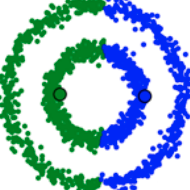
\includegraphics[width=0.15\linewidth]{2a.png} &
			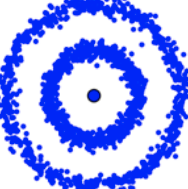
\includegraphics[width=0.15\linewidth]{2b.png} &
			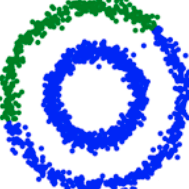
\includegraphics[width=0.15\linewidth]{2c.png} &
			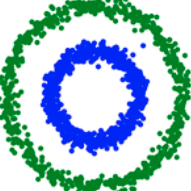
\includegraphics[width=0.15\linewidth]{2d.png} &
			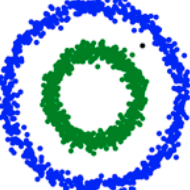
\includegraphics[width=0.15\linewidth]{2e.png} \\
			\hline
			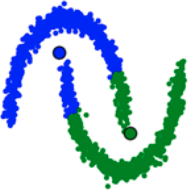
\includegraphics[width=0.15\linewidth]{2f.png} &
			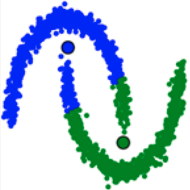
\includegraphics[width=0.15\linewidth]{2g.png} &
			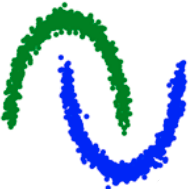
\includegraphics[width=0.15\linewidth]{2h.png} &
			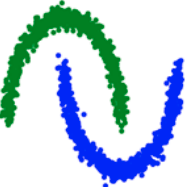
\includegraphics[width=0.15\linewidth]{2i.png} &
			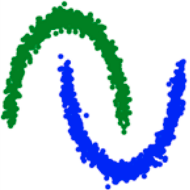
\includegraphics[width=0.15\linewidth]{2j.png} \\
			\hline
			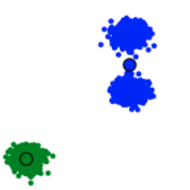
\includegraphics[width=0.15\linewidth]{2k.png} &
			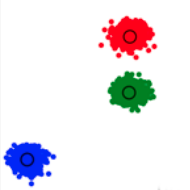
\includegraphics[width=0.15\linewidth]{2l.png} &
			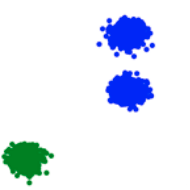
\includegraphics[width=0.15\linewidth]{2m.png} &
			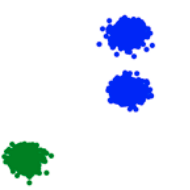
\includegraphics[width=0.15\linewidth]{2n.png} &
			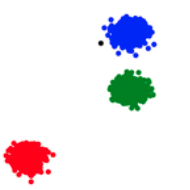
\includegraphics[width=0.15\linewidth]{2o.png} \\
			\hline
		\end{tabular}
	\end{figure}
\endgroup